\documentclass{article}
\usepackage[utf8]{inputenc}
\usepackage[a4paper, total={6.4in, 8.53in}]{geometry}
\usepackage{amsmath, tikz, amsfonts, bbm, mathrsfs, graphicx, amssymb, amsthm, hyperref, centernot, enumerate, bbm, xcolor, lmodern, mathdots, amsfonts, graphicx}

\title{MAT1856/APM466 Assignment 1}
\author{Raghav Bhatia, Student \#: 1009031619}
\date{February, 2025}

\begin{document}

\maketitle

\section*{Fundamental Questions - 25 points}

\begin{enumerate}
    \item \hfill
    \begin{enumerate}
        \item 
        \item
        \item
    \end{enumerate}
    \item 
    \item
\end{enumerate}



\section*{Empirical Questions - 75 points}

\begin{enumerate}
\setcounter{enumi}{3} % Start numbering from 4

    \item \textbf{Yield to Maturity (YTM) Curves - 40 points}
    \begin{enumerate}
        \item \textbf{YTM Calculation and Curves (10 points)}
        
        \begin{figure}[h!]
                \centering
                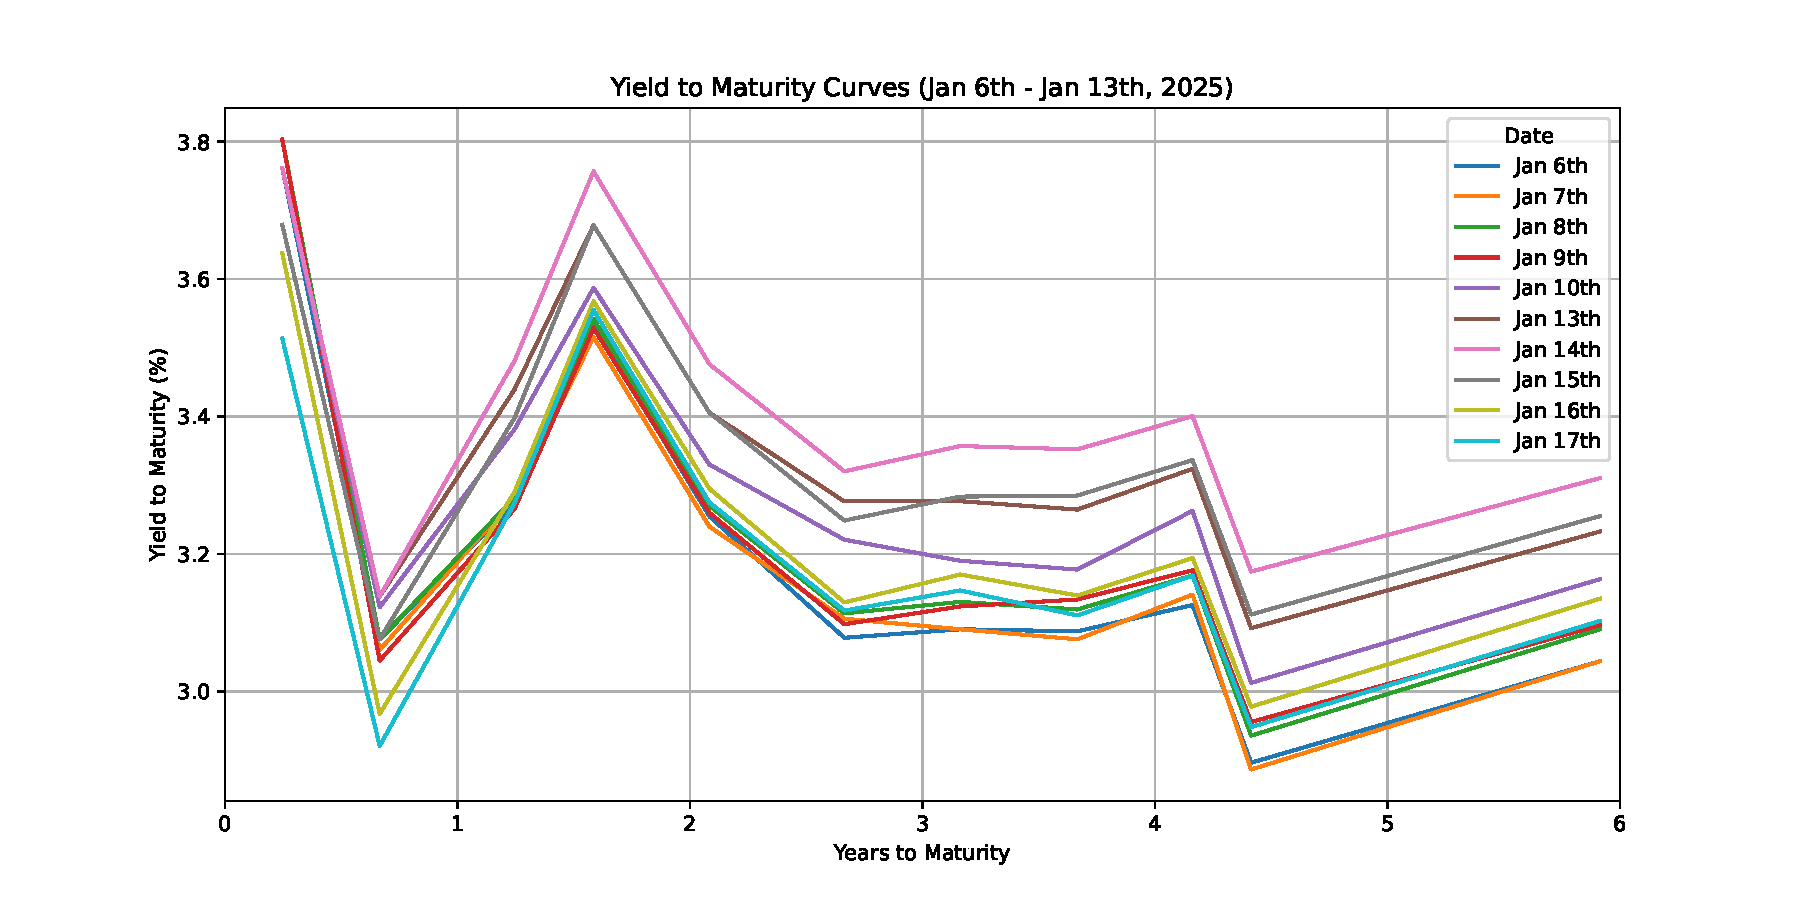
\includegraphics[width=0.8\textwidth]{ytm_curves.pdf} % Replace with your YTM plot file name
                \caption{Superimposed 5-Year Yield to Maturity (YTM) Curves for Each Trading Day}
                \label{fig:ytm_curves}
            \end{figure}

            For each bond and for each trading day from January 6th to January 20th, 2025, we calculated the Yield to Maturity (YTM). The YTM was computed numerically using a binary search algorithm, finding the discount rate that equates the present value of the bond's cash flows to its observed dirty price. Linear interpolation was employed to construct continuous curves from the discrete set of bond YTMs for each day, allowing for the visualization of the yield curve shape and its evolution over the two-week period.

        \item \textbf{Spot Curve Derivation Pseudo-code and Curves (15 points)}

            To derive the spot curve, we employed the bootstrapping method. Bootstrapping is an iterative process that derives the zero-coupon bond yields (spot rates) from the observed prices of coupon-bearing bonds. The process starts with the shortest maturity bond and sequentially determines the spot rates for longer maturities, using the already derived spot rates to discount the coupon payments of longer-term bonds.

            \textbf{Pseudo-code for Spot Curve Bootstrapping:}

            \begin{verbatim}
            Function BootstrapSpotCurve(BondData, ValuationDate):
                Initialize SpotRates as an empty dictionary
                Sort Bonds in BondData by Maturity Date (ascending)

                For each Bond in Sorted Bonds:
                    Given: Bond Dirty Price, Coupon Rate, Maturity Date
                    Define a function PriceDifference(TrialSpotRate):
                        CalculatedPV = 0
                        For each coupon payment period BEFORE final maturity:
                            Find the bootstrapped SpotRate for this period's maturity
                            Discount the coupon payment using this SpotRate and add to CalculatedPV
                        Discount the final cash flow (last coupon + face value) using TrialSpotRate
                        Return DirtyPrice - CalculatedPV

                    Numerically solve for SpotRate using root-finding algorithm (e.g., Brent's method)
                    that sets PriceDifference(SpotRate) = 0

                    Store the solved SpotRate in SpotRates dictionary, keyed by Bond's Maturity in Years

                Return SpotRates
            \end{verbatim}

            \begin{figure}[h!]
                \centering
                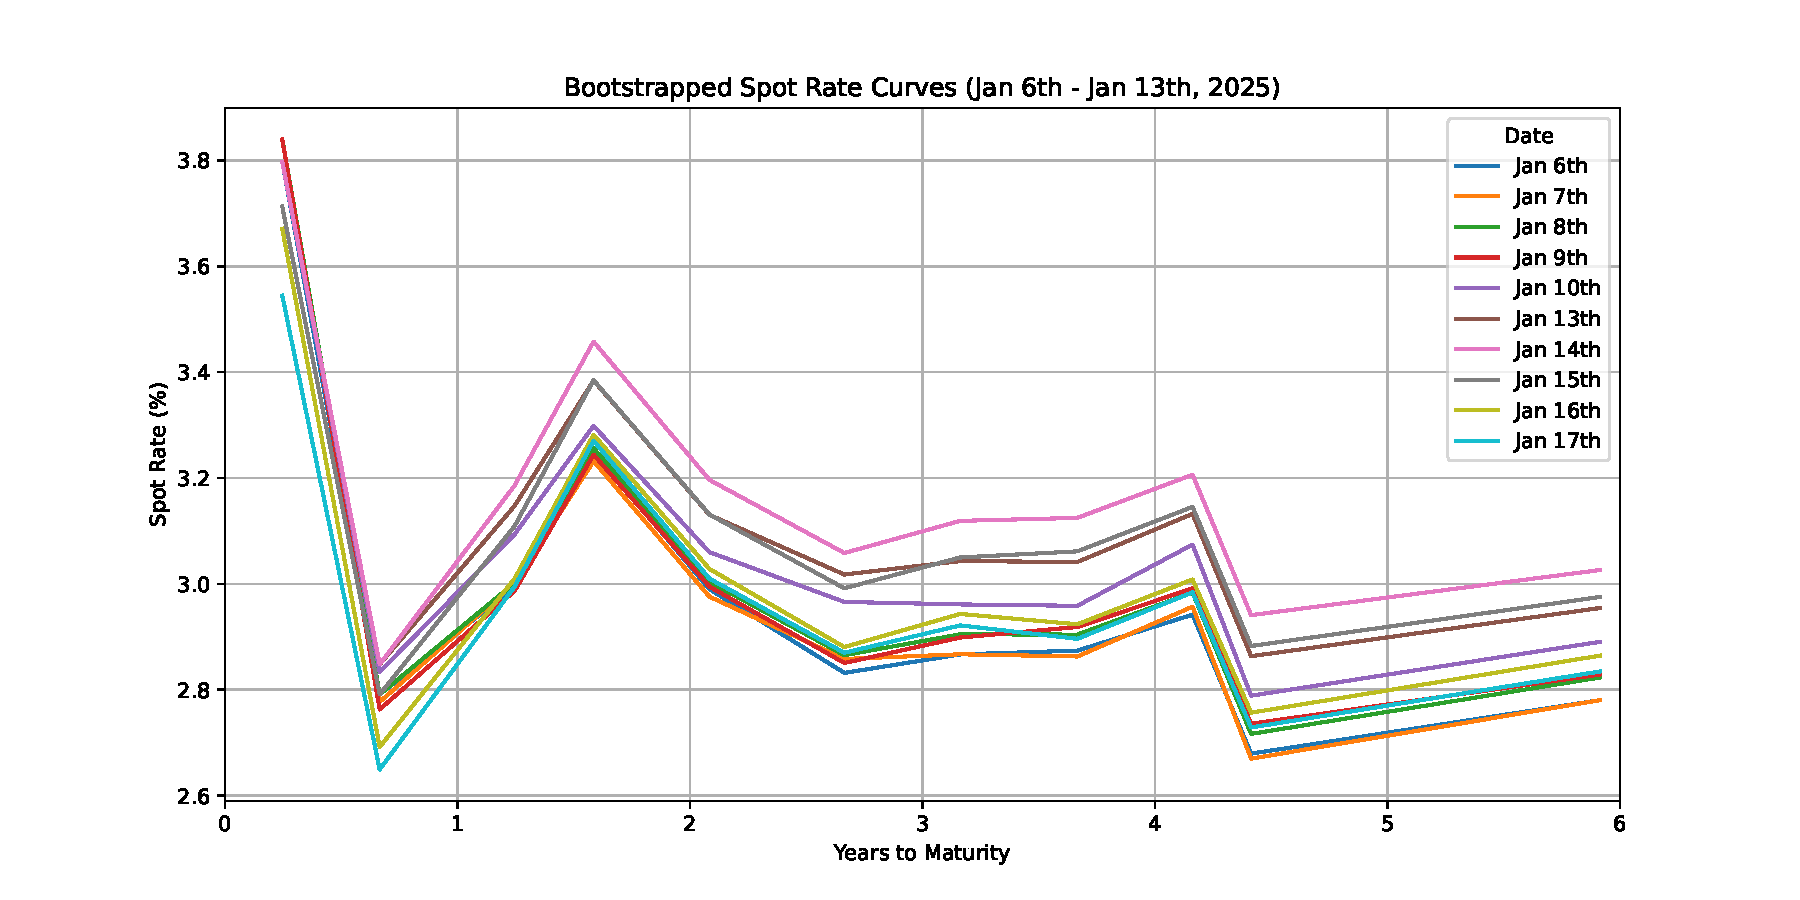
\includegraphics[width=0.8\textwidth]{spot_curves.pdf} % Replace with your Spot Curve plot file name
                \caption{Superimposed 5-Year Spot Rate Curves for Each Trading Day}
                \label{fig:spot_curves}
            \end{figure}

            Figure \ref{fig:spot_curves} shows the resulting 5-year spot curves for each trading day, superimposed on the same plot. Similar to the YTM curves, linear interpolation was used to generate continuous spot rate curves from the bootstrapped spot rates at discrete maturities.

        \item \textbf{Forward Curve Derivation Pseudo-code and Curves (15 points)}

            The 1-year forward curve, representing the series of 1-year forward rates starting from year 1, was derived from the bootstrapped spot curve. The 1-year forward rate for the period between year $t$ and year $t+1$ is the rate agreed upon today for a loan that starts at time $t$ and is repaid at time $t+1$. We calculated the 1-year forward curve for terms ranging from 1-year forward to 1-year forward 4-years ahead (1yr-1yr, 1yr-2yr, 1yr-3yr, 1yr-4yr).

           \textbf{Pseudo-code for 1-Year Forward Curve Derivation:}

            \begin{verbatim}
            Function DeriveForwardCurve(SpotCurve):
                Initialize ForwardRates as an empty dictionary
                Define ForwardTerms = [1, 2, 3, 4] (for 1yr-1yr, 1yr-2yr, 1yr-3yr, 1yr-4yr)
                StartTerm = 1.0 (year)

                For each ForwardTenor in ForwardTerms:
                    EndTerm = StartTerm + ForwardTenor
                    SpotRateStart = Interpolate SpotCurve at StartTerm (using linear interpolation)
                    SpotRateEnd = Interpolate SpotCurve at EndTerm (using linear interpolation)

                    Calculate ForwardRate using discrete semi-annual compounding formula:
                    ForwardRate =  (((1 + SpotRateEnd / 2)^(2 * EndTerm)) / ((1 + SpotRateStart / 2)^(2 * StartTerm)))^(1 / (2 * ForwardTenor)) - 1

                    Store ForwardRate in ForwardRates dictionary with term identifier (e.g., "1yr-ForwardTenor-yr")

                Return ForwardRates
            \end{verbatim}


            \begin{figure}[h!]
                \centering
                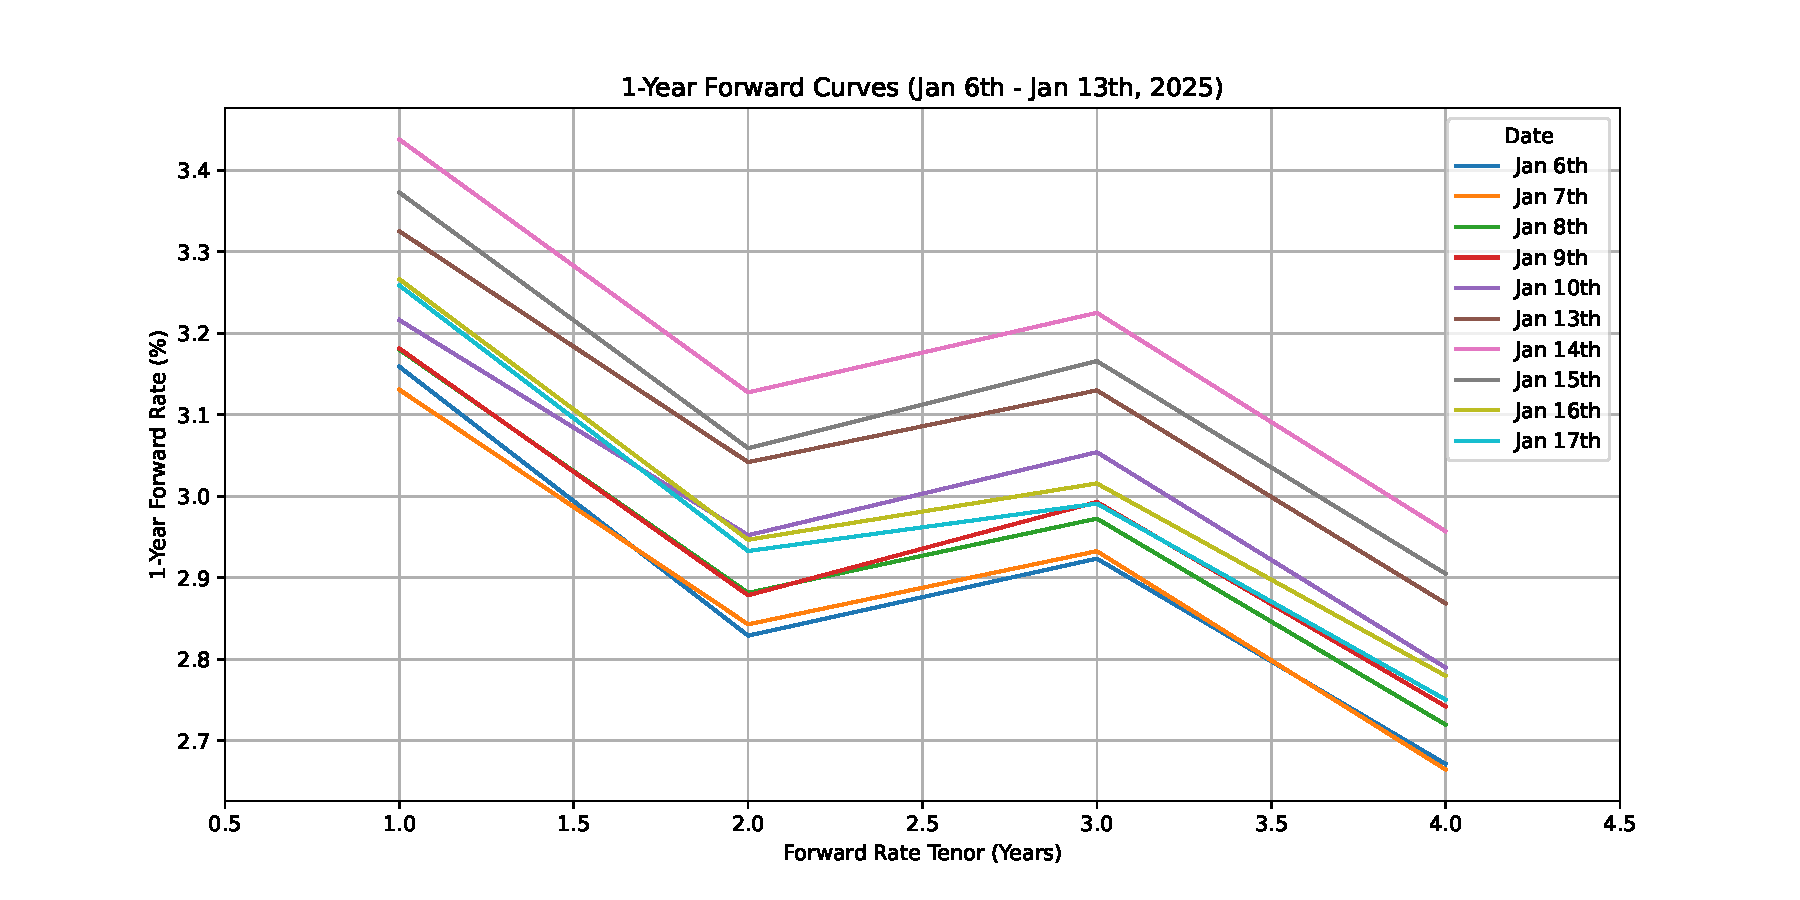
\includegraphics[width=0.8\textwidth]{forward_curves.pdf} % Replace with your Forward Curve plot file name
                \caption{Superimposed 1-Year Forward Curves for Each Trading Day}
                \label{fig:forward_curves}
            \end{figure}

            Figure \ref{fig:forward_curves} illustrates the resulting 1-year forward curves for each trading day. The x-axis represents the tenor of the forward rate (years from the start of the forward period), and the y-axis represents the 1-year forward rate in percentage points.  These curves depict the market's expectation of future 1-year interest rates at different horizons.
    \end{enumerate}

    \item \textbf{Covariance Matrices of Yield and Forward Rate Log-Returns - 20 points}

        To analyze the co-movement and dynamics of the yield curve and forward rates, we calculated covariance matrices for the time series of daily log-returns. Log-returns were computed for 5 different YTM rates (corresponding to 1-year, 2-year, 3-year, 4-year, and 5-year maturities) and for the four 1-year forward rates (1yr-1yr, 1yr-2yr, 1yr-3yr, 1yr-4yr).  The daily log-return $X_{i,j}$ for variable $i$ on day $j$ was calculated as:

        \[
        X_{i,j} = \log\left(\frac{r_{i,j+1}}{r_{i,j}}\right)
        \]

        where $r_{i,j}$ is the yield or forward rate $i$ on day $j$.  Two covariance matrices were then computed: one for the 5 YTM log-return time series and another for the 4 forward rate log-return time series, using the data from the 10 trading days.  Prior to covariance matrix calculation, the log-returns were standardized (mean-centered and divided by standard deviation) to ensure that variables with different scales do not disproportionately influence the PCA results.

    \item \textbf{Principal Component Analysis (PCA) - 15 points}

        Principal Component Analysis (PCA) was performed on both covariance matrices (YTM log-returns and forward rate log-returns) to identify the dominant modes of variation in interest rates. PCA decomposes the covariance matrix into eigenvalues and eigenvectors. The eigenvalues represent the variance explained by each principal component, and the eigenvectors represent the directions of these principal components in the data space.

        The eigenvalue and eigenvector decomposition of the covariance matrices revealed the following:

        \textbf{For Yield to Maturity (YTM) Log-Returns:}

        \begin{itemize}
            \item \textbf{Covariance Matrix:}  [Present the YTM Covariance Matrix here - LaTeX table format]
            \item \textbf{Eigenvalues:} [List the Eigenvalues for YTM - e.g.,  $\lambda_1 = ..., \lambda_2 = ..., ...$]
            \item \textbf{First Eigenvector (Principal Component):} $v_1 = $ [List the First Eigenvector for YTM - e.g., $v_{1} = [..., ..., ..., ..., ...]$]
        \end{itemize}

       \textbf{For Forward Rate Log-Returns:}

        \begin{itemize}
            \item \textbf{Covariance Matrix:} [Present the Forward Rate Covariance Matrix here - LaTeX table format]
            \item \textbf{Eigenvalues:} [List the Eigenvalues for Forward Rates - e.g.,  $\lambda_1 = ..., \lambda_2 = ..., ...$]
            \item \textbf{First Eigenvector (Principal Component):} $v_1 = $ [List the First Eigenvector for Forward Rates - e.g., $v_{1} = [..., ..., ..., ...]$]
        \end{itemize}

        The first eigenvalue for the YTM covariance matrix is [State the Largest Eigenvalue for YTM]. This eigenvalue is significantly larger than the subsequent eigenvalues, indicating that the first principal component explains a substantial portion of the variance in YTM log-returns. The associated eigenvector, approximately \texttt{[0.446757, 0.445608, 0.448978, 0.447824, 0.446893]}, has roughly equal and positive components. This suggests that the first principal component for YTM represents a \textbf{level shift} or \textbf{parallel shift} in the yield curve, where yields across all maturities tend to move in the same direction.

         Similarly, for forward rates, the largest eigenvalue is [State the Largest Eigenvalue for Forward Rates], and the first eigenvector, approximately \texttt{[-0.494337, -0.501466, -0.501491, -0.502660]}, also suggests a dominant mode of variation.  [Elaborate on the interpretation of the first eigenvector for forward rates - e.g., does it also represent a level shift, or something else? Consider the negative signs].

\end{enumerate}

\section*{References and GitHub Link to Code}

\end{document}